\documentclass[border=10pt]{standalone}
\usepackage{tikz}
\usetikzlibrary{shapes.geometric, arrows.meta, positioning, fit, backgrounds, calc}

\definecolor{prismaBlue}{RGB}{31, 73, 125}
\definecolor{prismaMid}{RGB}{68, 114, 196}
\definecolor{prismaLight}{RGB}{221, 235, 247}

\tikzset{
  mainbox/.style={
    rectangle, rounded corners=4pt,
    draw=prismaMid, line width=1.2pt,
    fill=prismaLight,
    text width=5.0cm, align=center,
    font=\small, inner sep=8pt,
    minimum height=1.2cm
  },
  sidebox/.style={
    rectangle, rounded corners=4pt,
    draw=prismaMid, line width=1.2pt,
    fill=white,
    text width=5.8cm, align=left,
    font=\small, inner sep=8pt
  },
  sectionlabel/.style={
    rectangle, fill=prismaBlue, text=white,
    font=\small\bfseries, rotate=90,
    inner sep=6pt, minimum height=1cm, align=center
  },
  myarrow/.style={-Stealth, line width=1.2pt, color=prismaBlue},
  sectionbg/.style={fill=prismaLight, draw=none, rounded corners=6pt}
}

\begin{document}
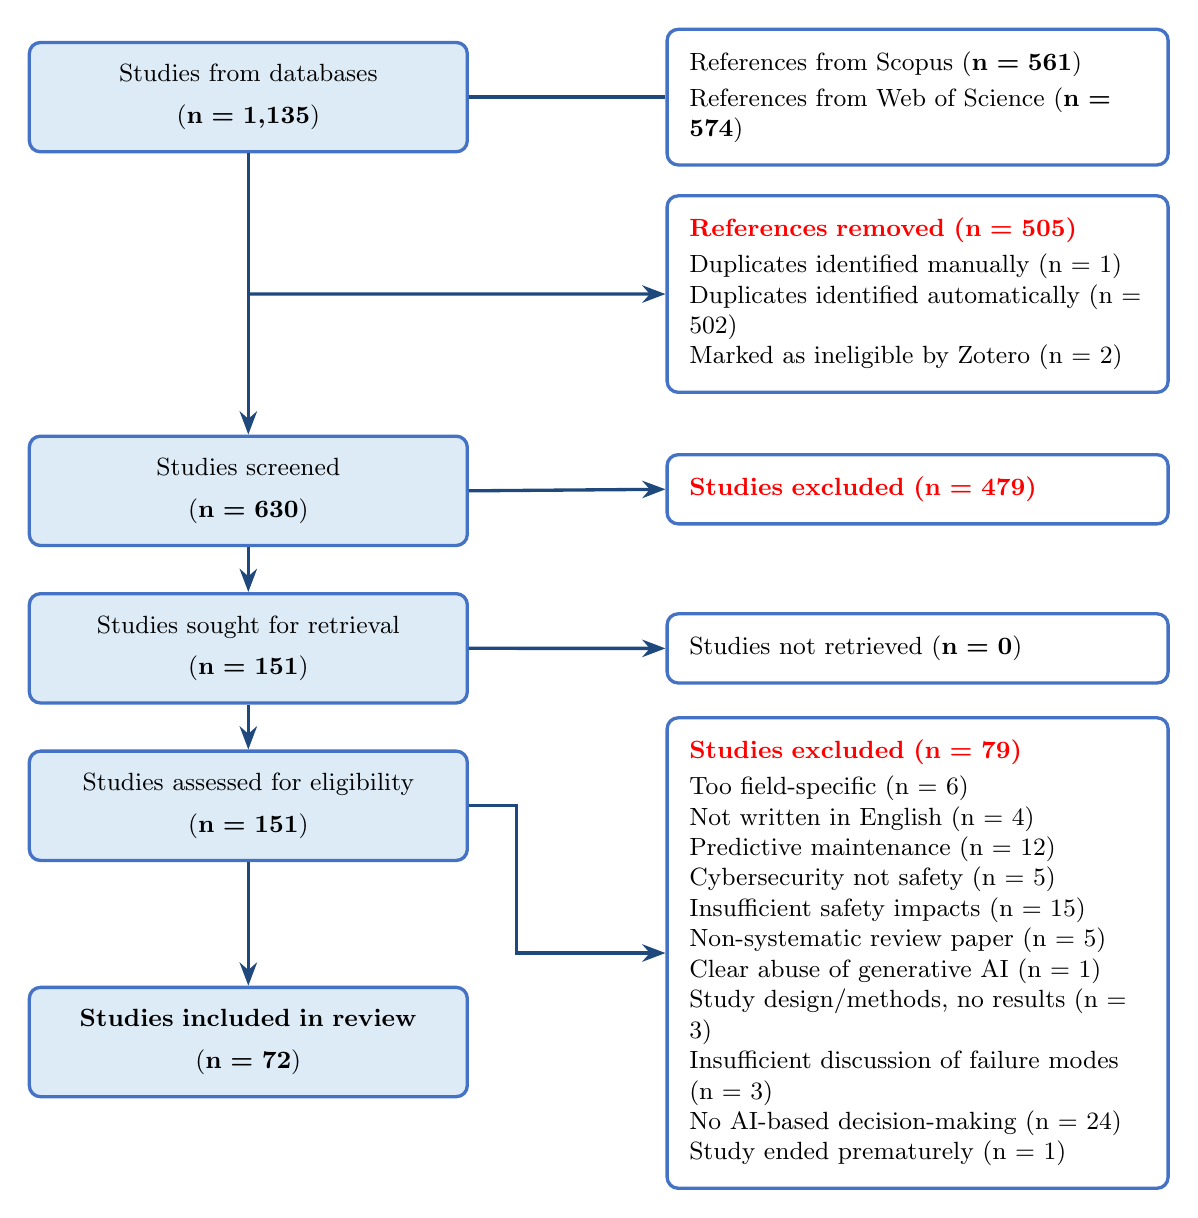
\begin{tikzpicture}

\def\leftX{0}
\def\rightX{8.5}

%% LEFT COLUMN
\node[mainbox] (databases) at (\leftX, 0) {
  Studies from databases\\[4pt](\textbf{n = 1,135})
};
\node[mainbox] (screened) at (\leftX, -5.0) {
  Studies screened\\[4pt](\textbf{n = 630})
};
\node[mainbox] (retrieval) at (\leftX, -7) {
  Studies sought for retrieval\\[4pt](\textbf{n = 151})
};
\node[mainbox] (eligibility) at (\leftX, -9) {
  Studies assessed for eligibility\\[4pt](\textbf{n = 151})
};
\node[mainbox] (included) at (\leftX, -12.0) {
  \textbf{Studies included in review}\\[4pt](\textbf{n = 72})
};

%% RIGHT COLUMN — each box anchored below the previous one
\node[sidebox] (breakdown) at (\rightX, 0) {
  References from Scopus (\textbf{n = 561})\\[2pt]
  References from Web of Science (\textbf{n = 574})
};
\node[sidebox, below=0.35cm of breakdown] (removed) {
  \textcolor{red}{\textbf{References removed (n = 505)}}\\[2pt]
  Duplicates identified manually (n = 1)\\
  Duplicates identified automatically (n = 502)\\
  Marked as ineligible by Zotero (n = 2)
};
\node[sidebox, below=0.75cm of removed] (excluded1) {
  \textcolor{red}{\textbf{Studies excluded (n = 479)}}
};
\node[sidebox, below=1.1cm of excluded1] (notretrieved) {
  Studies not retrieved (\textbf{n = 0})
};
\node[sidebox, below=0.4cm of notretrieved] (excluded2) {
  \textcolor{red}{\textbf{Studies excluded (n = 79)}}\\[2pt]
  Too field-specific (n = 6)\\
  Not written in English (n = 4)\\
  Predictive maintenance (n = 12)\\
  Cybersecurity not safety (n = 5)\\
  Insufficient safety impacts (n = 15)\\
  Non-systematic review paper (n = 5)\\
  Clear abuse of generative AI (n = 1)\\
  Study design/methods, no results (n = 3)\\
  Insufficient discussion of failure modes (n = 3)\\
  No AI-based decision-making (n = 24)\\
  Study ended prematurely (n = 1)
};

%% ARROWS
\draw[myarrow] (databases.south) -- (screened.north)
  node[midway] (joint) {};
\draw[color=prismaBlue, line width=1.2pt] (databases.east) -- (breakdown.west);
\draw[myarrow] (joint.center) -- (removed.west);
\draw[myarrow] (screened.south) -- (retrieval.north);
\draw[myarrow] (retrieval.south) -- (eligibility.north);
\draw[myarrow] (eligibility.south) -- (included.north);


% removed -> screened
% \draw[myarrow] (removed.west) -- ++(-0.6,0) |- (screened.east);

% screened -> excluded1
\draw[myarrow] (screened.east) -- (excluded1.west);

% retrieval -> notretrieved
\draw[myarrow] (retrieval.east) -- (notretrieved.west);

% eligibility -> excluded2
\draw[myarrow] (eligibility.east) -- ++(0.6,0) |- (excluded2.west);

%% BACKGROUND PANELS
% \begin{scope}[on background layer]
%   \node[sectionbg, fit=(databases)(breakdown)(removed), inner sep=14pt] (idpanel) {};
%   \node[sectionbg, fit=(screened)(retrieval)(eligibility)(excluded1)(notretrieved)(excluded2), inner sep=14pt] (screenpanel) {};
%   \node[sectionbg, fit=(included), inner sep=14pt] (incpanel) {};
% \end{scope}

%% LABELS
% \node[sectionlabel, left=0.35cm of idpanel] {Identification};
% \node[sectionlabel, left=0.35cm of screenpanel] {Screening};
% \node[sectionlabel, left=0.35cm of incpanel] {Included};

\end{tikzpicture}
\end{document}
